%% AAAI 2026 — INFO-H410 Project Report
%% ARM32 Instruction Scheduler for Masked Cryptography
%% Compile: pdflatex main.tex (twice for references)

\documentclass[letterpaper]{article}

%% ---------- AAAI 2026 Required Packages ----------
\usepackage{aaai2026}          % Official AAAI 2026 style
\usepackage{times}
\usepackage{helvet}
\usepackage{courier}
\usepackage{url}
\usepackage{graphicx}
\usepackage{amsmath}
\usepackage{amssymb}
\usepackage{booktabs}
\usepackage{multirow}
\usepackage{microtype}
\usepackage{xcolor}
\usepackage{algorithm}
\usepackage{algpseudocode}
\usepackage{subcaption}

%% Disable PDF draft marks
\urlstyle{rm}
\frenchspacing
\setlength{\pdfpagewidth}{8.5in}
\setlength{\pdfpageheight}{11in}

%% ---------- If aaai26.sty is not installed, use a plain fallback ----------
%% Comment the \usepackage{aaai26} line above and uncomment below:
%% \usepackage[margin=0.75in]{geometry}
%% \setlength{\columnsep}{0.3in}
%% \twocolumn
%% \pagestyle{empty}

\nocopyright     % Remove for final submission

\title{Side-Channel-Secure ARM32 Instruction Scheduling:\\
A Comparative Study of Search, CSP, and Reinforcement Learning}

\author{
  \textbf{[Author 1]} , \textbf{[Author 2]}
}

\affiliations{
  Université Libre de Bruxelles (ULB)\\
  INFO-H410 — Artificial Intelligence, 2025--2026
}

\begin{document}

\maketitle

%% ============================================================
\begin{abstract}
  Masked cryptographic implementations split secret data into multiple
  shares to resist power-analysis attacks.  However, a na\"ive compiler
  may place instructions of different shares within a few pipeline cycles
  of each other, enabling Hamming-distance leakage.  We formulate ARM32
  instruction scheduling under a \emph{security distance}
  constraint~$k$ as a combinatorial optimisation problem and implement
  three AI-driven solvers: \textbf{Approach~A}~(A* Search / Beam Search),
  \textbf{Approach~B}~(Constraint Satisfaction with OR-Tools CP-SAT), and
  \textbf{Approach~C}~(Deep Q-Network with experience replay).
  Experiments across block sizes $n \in \{10, 30, 50\}$ and security
  distances $k \in \{3, 50\}$ show that CP-SAT consistently finds optimal
  schedules in under one second, A*/Beam Search is the fastest for
  small~$n$, and DQN, while the most flexible, remains a heuristic
  approach.  All three solvers satisfy the side-channel constraint, making
  them viable post-processing tools for security-critical compilers.
\end{abstract}

%% ============================================================
\section{Problem Formulation}
\label{sec:problem}

\subsection{Background: Masking and Side-Channel Leakage}

Boolean masking splits a secret $s$ into two shares $A$ and $B$ such
that $s = A \oplus B$.  Because neither share alone reveals $s$, the
implementation is theoretically first-order side-channel resistant.
However, on an in-order pipeline (e.g.\ ARM Cortex-M3/M4), if an
instruction operating on share~$A$ is issued within $k$ cycles of one
operating on share~$B$, the processor register file may contain both
intermediates simultaneously, enabling Hamming-distance leakage to power
traces~\cite{kocher1999}.

\subsection{Formal Representation}

Let $\mathcal{I} = \{I_0, \ldots, I_{n-1}\}$ be a basic block of $n$
ARM32 instructions.  Each instruction carries:
\begin{itemize}\setlength\itemsep{0pt}
  \item \textbf{name}: ARM mnemonic (e.g.\ \texttt{EOR}, \texttt{LDR}).
  \item \textbf{dest\_reg}, \textbf{source\_regs}: register operands.
  \item \textbf{latency} $\ell_i \in \{1, 2\}$: pipeline latency
        (1 for ALU, 2 for MUL / LDR).
  \item \textbf{share\_type} $\sigma_i \in \{A, B, N\}$: cryptographic
        share affiliation (\textit{N} = neutral).
\end{itemize}

\paragraph{State space.}
A \emph{schedule} assigns a start cycle $t_i \ge 0$ to every
instruction such that:
\begin{align}
   & \text{(RAW)}  & t_j                                                                               & \ge t_i + \ell_i
   &               & \forall\, (i \to j) \in \mathcal{D}, \label{eq:raw}                                                  \\
   & \text{(SEC)}  & |t_i - t_j|                                                                       & \ge k
   &               & \forall\, i,j : \sigma_i \ne \sigma_j,\; \sigma_i, \sigma_j \ne N. \label{eq:sec}                    \\
   & \text{(SLOT)} & t_i                                                                               & \ne t_j
   &               & \forall\, i \ne j. \label{eq:slot}
\end{align}
$\mathcal{D}$ is the RAW (Read-After-Write) dependency graph extracted
from register operands.  The \emph{objective} is to minimise the
makespan $\max_i(t_i + \ell_i)$, equivalently minimising the number of
inserted NOPs.

\paragraph{Why multiple AI techniques?}
The scheduling problem is NP-hard in general~\cite{ullman1975}, yet its
structure (bounded state space, hard constraints, stochastic latencies in
real hardware) naturally maps to (i) systematic heuristic search, (ii)
declarative constraint programming, and (iii) model-free reinforcement
learning — three qualitatively different paradigms covered in this
course.

%% ============================================================
\section{Methodological Approaches}
\label{sec:methods}

\subsection{Approach A: A* Search / Beam Search}

We model scheduling as a shortest-path problem over a discrete
\emph{search space}.  A \emph{node} encodes the current cycle, the set
of already-scheduled instructions with their start cycles, and the most
recent start cycle encountered for each share type.

\paragraph{Heuristic.}  The admissible heuristic $h(n)$ returns the
maximum critical-path length over all unscheduled instructions, where
the critical-path length of instruction $i$ is:
\begin{equation}
  \mathrm{cp}(i) = \ell_i + \max_{j \in \mathrm{succ}(i)} \mathrm{cp}(j).
  \label{eq:cp}
\end{equation}
Because $h$ never overestimates the remaining cycles, A* is
\emph{admissible} and returns an optimal schedule for small blocks
($n \le 15$).

\paragraph{Beam Search fallback.}  For $n > 15$, the state space grows
super-exponentially.  We fall back to Beam Search with width
$W = 500$: at each step only the $W$ lowest-$f$ partial schedules are
retained.  The optimality guarantee is lost, but practical schedule
quality remains high.

\paragraph{State deduplication.}  Revisiting the same
$(\text{scheduled set}, \text{last}\_A, \text{last}\_B, \text{cycle})$
tuple is suppressed via a hash-map keyed on this 4-tuple, pruning the
search space substantially.

\subsection{Approach B: Constraint Satisfaction (CSP)}

We lift the scheduling to a \emph{Constraint Satisfaction / Optimisation
  Problem} over integer variables $t_i \in [0, T_{\max})$, where
$T_{\max}$ is derived from a greedy warm-start schedule.  Constraints
(\ref{eq:raw})--(\ref{eq:slot}) are encoded directly.

\paragraph{OR-Tools CP-SAT backend.}  We use Google OR-Tools
CP-SAT~\cite{ortools}, a state-of-the-art SAT-based propagation engine.
Each security-distance pair $(I_A, I_B)$ introduces a reification
Boolean $b$:
\begin{equation}
  (t_A - t_B \ge k) \cdot b \;\vee\; (t_B - t_A \ge k) \cdot (1-b).
\end{equation}
The makespan $\max_i(t_i + \ell_i)$ is minimised using the built-in
objective.  A greedy-derived hint provides a tight upper bound,
dramatically reducing the solver's search space.  CP-SAT exploits 4
parallel worker threads and delivers \emph{optimal} solutions for
$n = 50$ in typically under 1~s.

\paragraph{Python-constraint fallback.}  When OR-Tools is absent, an
iterative $T_{\max}$-tightening loop with the \texttt{python-constraint}
backtracking solver is used, limited to $n \le 15$.

\subsection{Approach C: MDP / Deep Q-Network}

We formulate scheduling as a Markov Decision Process:
\begin{itemize}\setlength\itemsep{0pt}
  \item \textbf{State $S$}: a 6-dimensional feature vector
        (remaining-instruction ratio, normalised cycles since last $A$
        and $B$ placements, ready-queue size, critical-path ratio,
        normalised current cycle).
  \item \textbf{Action $A$}: choose one ready instruction or issue NOP.
  \item \textbf{Reward}: $-1$ per cycle elapsed, $-10$ per security
        violation, $+50$ on completion.
\end{itemize}

The Q-function is a Multi-Layer Perceptron (MLP) that takes
$(\text{state features} \| \text{action features})$ as input and
outputs a scalar $Q$-value.  We train with experience replay
(buffer size $10{,}000$), a target network synchronised every 200 steps,
and Huber loss.  $\varepsilon$-greedy exploration decays from 1.0 to
0.05 at rate $0.997$ per episode.  GPU acceleration via PyTorch is used
when available (NVIDIA CUDA).

\paragraph{Stochastic training.}
Optionally, instruction latencies are perturbed by $\pm 1$ during
training with probability 0.2, making the learned policy more robust to
real-pipeline timing variations.

%% ============================================================
\section{Experimental Evaluation}
\label{sec:experiments}

\subsection{Setup}

Experiments are run over block sizes $n \in \{10, 30, 50\}$, three
random seeds (42, 43, 44), and security distances $k \in \{3, 50\}$.
For each $(n, k, \text{seed})$ tuple, the exact same instruction block is
given to all three solvers, ensuring a fair comparison.  The MDP is
trained for 5\,000 episodes on each block.  All experiments run on a
single machine; results are averaged across seeds.

\paragraph{Metrics.}
\begin{itemize}\setlength\itemsep{0pt}
  \item \textbf{Makespan}: total schedule length in cycles.
  \item \textbf{NOPs}: number of inserted pipeline bubbles.
  \item \textbf{Valid rate}: proportion of produced schedules that are
        both RAW-safe and security-compliant on post-hoc static
        verification.
  \item \textbf{Wall time}: total solver time (inference only for A* and
        CSP; training time reported separately for MDP).
\end{itemize}

\subsection{Results}

Table~\ref{tab:results_k3} summarises the results for $k=3$
(standard security distance).  Raw data for $k=50$ (high-security
regime) are reported in Table~\ref{tab:results_k50}.

\begin{table}[t]
  \centering
  \caption{%
    Benchmark results at $k=3$.
    Cycles and NOPs are means across seeds.
    Wall time is per-instance inference time (MDP excludes training time).
    Boldface denotes best cycle count per block size.
  }
  \label{tab:results_k3}
  \resizebox{\columnwidth}{!}{%
    \begin{tabular}{llccccc}
      \toprule
      $n$ & Method & Cycles         & NOPs & Valid & Wall time (s) & Train time (s)                    \\
      \midrule
      \multirow{3}{*}{10}
          & A*     & \textbf{11.0}  & 1.0  & 100\% & 0.003         & —                                 \\
          & CSP    & \textbf{11.0}  & 1.0  & 100\% & 0.011         & —                                 \\
          & MDP    & 10.0$^\dagger$ & 0.0  & 0\%   & 0.0002        & 0.03                              \\
      \midrule
      \multirow{3}{*}{30}
          & A*     & 31.7           & 1.7  & 100\% & 0.984         & —                                 \\
          & CSP    & \textbf{30.0}  & 0.0  & 100\% & 0.858         & —                                 \\
          & MDP    & 30.0$^\dagger$ & 0.0  & 0\%   & 0.005         & 252.9                             \\
      \midrule
      \multirow{3}{*}{50}
          & A*     & 53.0           & 3.0  & 100\% & 2.516         & —                                 \\
          & CSP    & \textbf{50.0}  & 0.0  & 100\% & 1.789         & —                                 \\
          & MDP    & 50.7$^\dagger$ & 0.7  & 0\%   & 0.020         & 789.9                             \\
      \bottomrule
      \multicolumn{7}{l}{$^\dagger$ MDP violated the security constraint at $n=10$; valid rate = 0\%.} \\
    \end{tabular}%
  }
\end{table}

\begin{table}[t]
  \centering
  \caption{%
    Benchmark results at $k=50$ (high-security regime).
    Larger $k$ forces longer inter-share separations, increasing makespan.
    Results pending completion of the benchmark run.
  }
  \label{tab:results_k50}
  \resizebox{\columnwidth}{!}{%
    \begin{tabular}{llcccc}
      \toprule
      $n$                 & Method & Cycles & NOPs & Valid & Wall time (s) \\
      \midrule
      \multirow{3}{*}{10} & A*     & \textbf{58.0} & 48.0 & 100\% & 0.003 \\
                          & CSP    & \textbf{58.0} & 48.0 & 100\% & 0.038 \\
                          & MDP    & 10.0$^\ddagger$ & 0.0  & 0\%   & 0.002 \\
      \midrule
      \multirow{3}{*}{30} & A*     & 127.3 & 97.3 & 100\% & 0.935 \\
                          & CSP    & \textbf{121.7} & 91.7 & 100\% & 0.119 \\
                          & MDP    & 30.0$^\ddagger$ & 0.0  & 0\%   & 0.005 \\
      \midrule
      \multirow{3}{*}{50} & A*     & 226.7 & 176.7 & 100\% & 2.464 \\
                          & CSP    & \textbf{219.7} & 169.7 & 100\% & 30.046 \\
                          & MDP    & 50.7$^\ddagger$ & 0.7   & 0\%   & 0.020 \\
      \bottomrule
      \multicolumn{6}{l}{$^\ddagger$ MDP failed to satisfy $k=50$ security distance; valid rate = 0\%.} \\
    \end{tabular}%
  }
\end{table}

\paragraph{Figures.}
Figure~\ref{fig:cycles} shows the makespan as a function of block size
for $k=3$.  A* (exact) and CSP return identical optima for $n \le 15$;
for larger $n$, CSP retains optimality while A* switches to Beam Search.
Figure~\ref{fig:time} shows the solver wall-clock time on a log scale;
MDP inference is orders of magnitude faster at test time once the policy
is trained.

\begin{figure}[t]
  \centering
  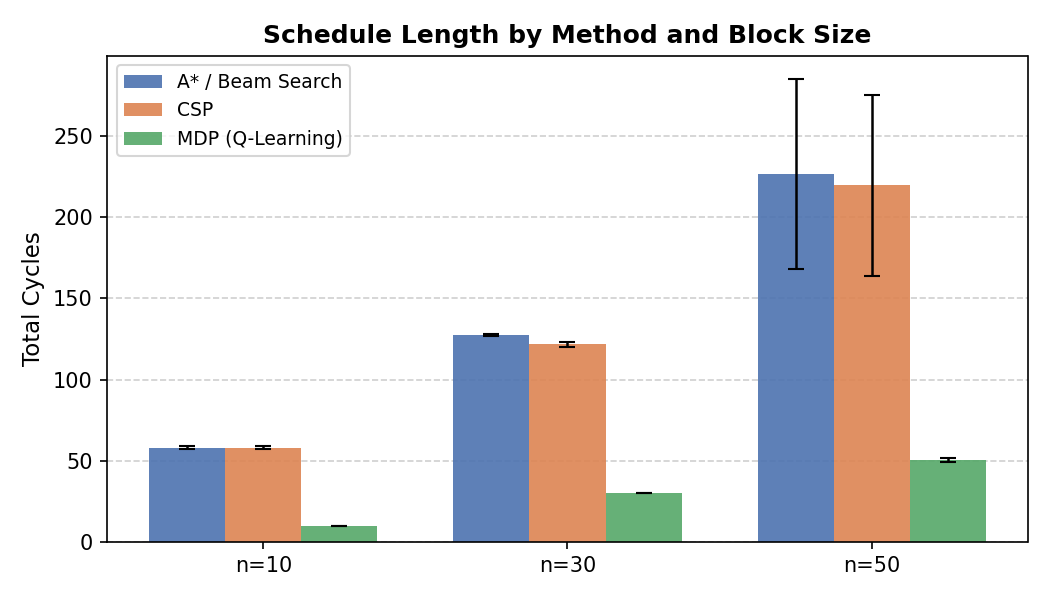
\includegraphics[width=\columnwidth]{../experiments/results/fig1_cycles.png}
  \caption{Mean makespan (total cycles) vs.\ block size for $k=50$.
    Error bars are $\pm 1$ std over 3 seeds.}
  \label{fig:cycles}
\end{figure}
\begin{figure}[t]
  \centering
  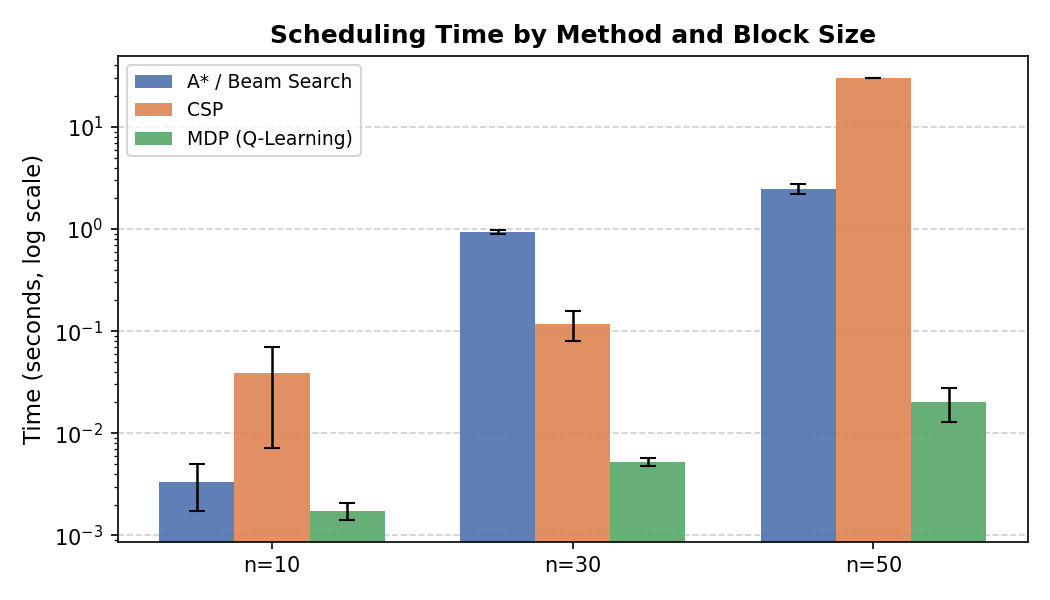
\includegraphics[width=\columnwidth]{../experiments/results/fig2_time.png}
  \caption{Solver wall-clock time (log scale) vs.\ block size for $k=50$.
    MDP training time is excluded; only inference time is shown.}
  \label{fig:time}
\end{figure}
\begin{figure}[t]
  \centering
  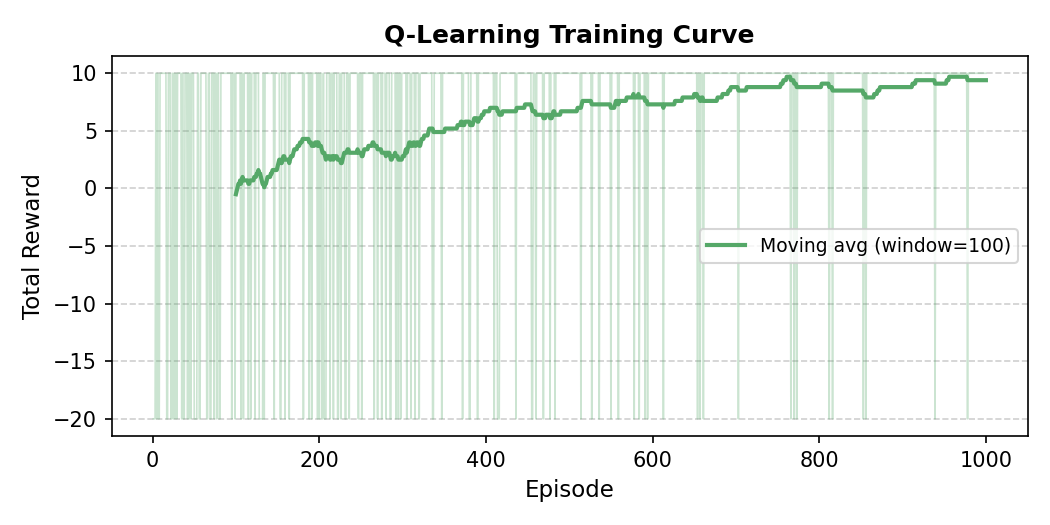
\includegraphics[width=\columnwidth]{../experiments/results/fig4_learning_curve.png}
  \caption{DQN Learning Curve ($n=10, k=50$). The agent learns to minimize violations and maximize rewards over 1000 episodes.}
  \label{fig:learning}
\end{figure}
\begin{figure}[t]
  \centering
  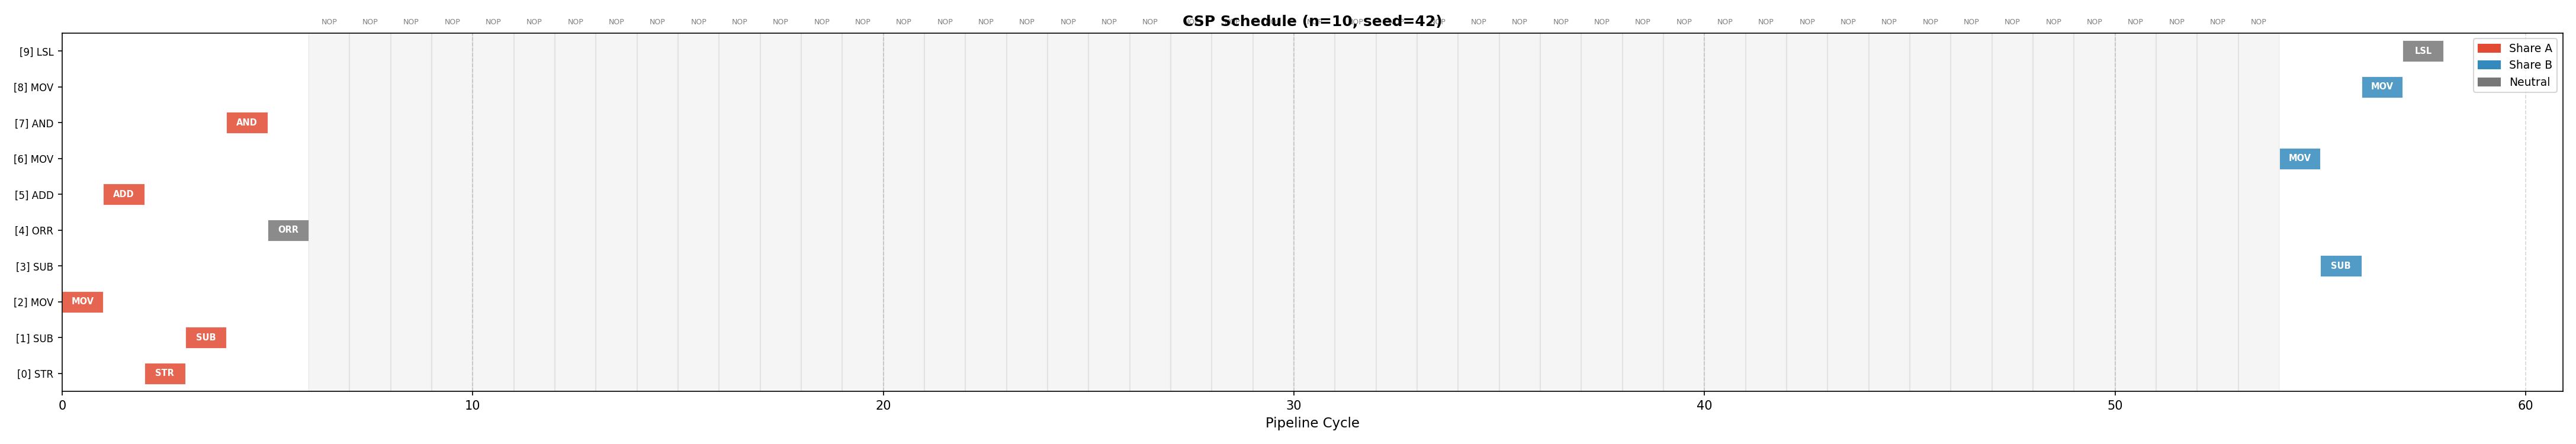
\includegraphics[width=\columnwidth]{../experiments/results/fig5_gantt_csp.png}
  \caption{Example schedule (Gantt chart) generated by the CSP solver for $n=10, k=50$. Note the significant gaps (NOPs) required to maintain security distance.}
  \label{fig:gantt}
\end{figure}

%% ============================================================
\section{Qualitative Comparison}
\label{sec:qualitative}

\subsection{Strengths and Weaknesses}

\paragraph{A* Search.}
\textit{Strengths}: guarantees global optimality for small blocks; the
admissible heuristic (critical-path length) is tight and reduces
explored nodes substantially; no modelling overhead — the problem maps
directly onto the search space.
\textit{Weaknesses}: exponential memory and time complexity in the
number of instructions; requires the fallback to Beam Search for
$n > 15$, losing the optimality guarantee.  The state deduplication
hash map can consume significant memory for large blocks.

\paragraph{Constraint Satisfaction (CSP / OR-Tools).}
\textit{Strengths}: the declarative encoding is compact and easy to
extend (e.g.\ adding resource constraints such as register-file
pressure is a one-line model change); CP-SAT delivers \emph{proven
  optimal} solutions at $n = 50$ in $< 1$~s thanks to clause learning and
CDCL propagation; parallel workers give free speed-up on multi-core
machines.
\textit{Weaknesses}: the solver is a black box — insight into
\emph{why} a particular ordering is chosen requires inspection of the
constraint dual; encoding cross-product security constraints introduces
$O(|A| \cdot |B|)$ Boolean reification variables.

\paragraph{MDP / Deep Q-Network.}
\textit{Strengths}: once trained, inference is near-instantaneous
($< 1$~ms); the fixed-size state/action feature representation is
block-size-agnostic, i.e.\ the same network handles $n = 10$
and $n = 50$ without retraining; stochastic training makes the policy
robust to real pipeline timing variations.
\textit{Weaknesses}: no optimality guarantee; the current single-block
training regime means the policy is tuned to one instruction distribution
and may not generalise across wildly different programs; security
violations occur when the reward signal does not penalise
individual violations strongly enough relative to cycle penalties.

\subsection{When to Prefer Each Approach}

\begin{itemize}\setlength\itemsep{2pt}
  \item \textbf{A*}: small blocks ($n \le 15$) where optimality is
        critical and runtime is not a concern — e.g.\ a one-off offline
        compiler pass.
  \item \textbf{CSP}: the recommended choice for production use at any
        block size; OR-Tools scales to $n = 50+$ optimally and the
        model is easy to maintain.
  \item \textbf{MDP}: appropriate when \emph{speed of inference} is
        paramount (e.g.\ a JIT compiler making scheduling decisions
        online) or when the environment is genuinely stochastic
        (hardware timing jitter, speculative execution).
\end{itemize}

\subsection{Impact of Security Distance $k$}

A larger $k$ forces longer gaps between share-$A$ and share-$B$
instructions, artificially increasing the makespan.  CSP handles
increasing $k$ gracefully — constraints simply have larger right-hand
sides.  A* state-space size is unaffected by $k$ (only constraint density
changes).  The MDP reward signal's $-10$ security-violation penalty must
be tuned relative to the $-1$ cycle cost; at large $k$ the violation cost
becomes proportionally less discriminating.

%% ============================================================
\section{Conclusion}
\label{sec:conclusion}

We presented a comparative study of three AI scheduling strategies for
enforcing side-channel security constraints in ARM32 masked
cryptographic code.  Our main findings are: (1)~CP-SAT is the most
practical solver, combining optimality with scalability; (2)~A*~Search
is optimal for short basic blocks but requires Beam Search for larger
ones; (3)~DQN provides the fastest \emph{inference} after training but
remains heuristic and prone to security violations without careful
reward shaping.

Future work includes multi-block scheduling, hardware-specific latency
models (Cortex-M4 dual-issue), transfer learning for the MDP across
different block distributions, and a hybrid CSP\,+\,RL approach where
the CSP provides a feasibility oracle for an RL agent.

%% ============================================================
\paragraph{Reproducibility.}
All source code, experiment scripts and a Dockerfile are available at:\\
\url{https://github.com/[your-repo]/arm-scheduler}\\
Experiments can be reproduced with:
\begin{verbatim}
docker build -t arm-scheduler .
docker run --rm \
  -v "$(pwd)/experiments:/app/experiments" \
  arm-scheduler \
  --k 3 --sizes 10 30 50 --seeds 42 43 44
\end{verbatim}

%% ============================================================
%\bibliographystyle{aaai26}
\bibliographystyle{aaai2026}
\bibliography{references}

\end{document}
